\f0\fs24 \cf0 % --- UNIVERSAL PREAMBLE BLOCK ---
\documentclass[11pt, a4paper]{article}
\usepackage[top=2.0cm, bottom=2.0cm, left=2.2cm, right=2.2cm]{geometry}
\usepackage{fontspec}
\usepackage[chinese, provide=*]{babel}

% 设置字体 - 使用 Noto 系列
\babelfont{rm}{Noto Sans CJK SC}
\babelfont{sf}{Noto Sans CJK SC}

% --- 颜色与设计包 ---
\usepackage{xcolor}
\usepackage{tikz}
\usetikzlibrary{patterns, shadows, calc, decorations.pathmorphing}
\usepackage[most]{tcolorbox}
\usepackage{enumitem}
\usepackage{hyperref}
\usepackage{parskip}
\usepackage{tabularx}
\usepackage{setspace}
\usepackage{graphicx}
\usepackage{longtable}
\usepackage{colortbl}
\usepackage{multicol}

% --- 增加全局行间距 ---
\linespread{1.5}

% --- 定义配色方案 ---
\definecolor{HealingPurple}{HTML}{6A75BA}  % 主标题色
\definecolor{OrchidPink}{HTML}{DDB6D3}     % 装饰粉
\definecolor{Periwinkle}{HTML}{B2B3DA}     % 装饰蓝
\definecolor{PaleRose}{HTML}{F2E6EB}       % 基础淡粉
\definecolor{PageBg}{HTML}{FFFCFD}         % 极淡背景
\definecolor{TextDark}{HTML}{555555}       % 正文深灰

% 极浅的边框颜色
\definecolor{SoftLieFrame}{HTML}{E0B0B0}   % 极浅红
\definecolor{SoftTruthFrame}{HTML}{B0BFE0} % 极浅蓝

% 应用背景色
\pagecolor{PageBg}
\color{TextDark}

% --- 自定义标题样式 ---
\usepackage{titlesec}

\newcommand\CloudSection[1]{%
    \vspace{0.5em}
    \begin{tikzpicture}
        \node[
            fill=PaleRose!40,
            rounded corners=10pt,
            inner sep=10pt,
            text width=\textwidth-20pt,
            align=left
        ] (box) {
            \textcolor{HealingPurple}{\Large\bfseries #1}
        };
        % 左侧柔和装饰条
        \draw[OrchidPink, line width=3pt, line cap=round] 
            ($(box.north west)+(0.1, -0.1)$) -- ($(box.south west)+(0.1, 0.1)$);
    \end{tikzpicture}%
    \vspace{0.2em}
}

\titleformat{\section}
{\normalfont}{}{0em}{\CloudSection}

\titleformat{\subsection}
{\color{HealingPurple}\large\bfseries}{}{0em}{}

% --- 附录盒子 ---
\newtcolorbox{softbox}[1][]{
    enhanced,
    colback=white,
    colframe=OrchidPink!50,
    title=#1,
    coltitle=white,
    fonttitle=\bfseries,
    attach boxed title to top left={yshift=-2mm, xshift=2mm},
    boxed title style={colback=OrchidPink!70, rounded corners},
    arc=3mm,
    boxrule=0.5mm,
    drop fuzzy shadow
}

% --- 列表设置 ---
\setlist[itemize]{label=\textcolor{OrchidPink}{\textbullet}, leftmargin=*, itemsep=2pt, topsep=2pt}
\setlist[enumerate]{label=\textcolor{HealingPurple}{\textbf{\arabic*.}}, leftmargin=*, itemsep=2pt, topsep=2pt}

% --- 文档开始 ---
\begin{document}

% --- 封面页 ---
\thispagestyle{empty}
\begin{center}
    \vspace*{4cm}
    
    % 标题区域
    \begin{minipage}{1.0\textwidth}
        \centering
        \resizebox{\textwidth}{!}{
            \bfseries\textcolor{HealingPurple}{CPTSD (复杂性创伤后应激障碍)}
        }\\[0.3cm]
        {\fontsize{32}{40}\bfseries\textcolor{HealingPurple}{自我疗愈指南}}
    \end{minipage}

    \vspace{2cm}

    % 装饰
    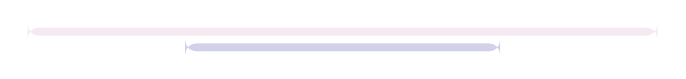
\begin{tikzpicture}
        \fill[OrchidPink!30, rounded corners] (0,0) rectangle (8, 0.1);
        \fill[Periwinkle!60, rounded corners] (2,-0.2) rectangle (6, -0.1);
    \end{tikzpicture}
    
    \vspace{3cm}
    
    % 引言文案
    \begin{minipage}{0.9\textwidth}
        \color{TextDark}
        \normalsize
        \raggedright 
        \setstretch{1.8}
        这份指南旨在为正在经历CPTSD症状(如情绪闪回、批判声音、抑郁感)的人士提供即时的心理学工具。请将此作为你的“安全地图”,下面让我们一起开启你的疗愈旅程
    \end{minipage}
    
    \vfill
\end{center}

\newpage

% --- 目录 ---
{
  \hypersetup{linkcolor=HealingPurple}
  \tableofcontents
}
\newpage

% --- 正文内容 ---

\section{第一部分:情绪闪回急救箱(13个步骤)}

当突然感到极度恐惧、羞耻、渺小或绝望时,请按顺序执行以下步骤。

\begin{enumerate}
    \item \textbf{命名与确认}
    \begin{itemize}
        \item 对自己说:“我正在经历情绪闪回。”
        \item 认知定位:承认现在的感觉(恐惧、被遗弃感)实际上是过去的记忆被激活了。你并没有真的回到过去,这只是过去的痛苦在当下的重演。
    \end{itemize}

    \item \textbf{确认安全}
    \begin{itemize}
        \item 提醒自己:“无论我感到多么害怕,其实我现在很安全。”
        \item 现实检验:你现在已经远离了童年时的那些危险。你现在处于成人身体中,你有能力保护自己。
    \end{itemize}

    \item \textbf{确立边界}
    \begin{itemize}
        \item 对内:提醒自己不必让每个人都喜欢你。
        \item 对外:你有权离开让你感到不安全的人或环境。如果当下环境触发了闪回,请暂时物理离开那个环境。
    \end{itemize}

    \item \textbf{安抚“内在小孩”}
    \begin{itemize}
        \item 对话:对自己受惊的内心说话:“我知道你现在很害怕/受伤/难过,但我在这里,我会一直陪着你,我会保护你。”
        \item 想象:想象一个理想的父母会如何安抚孩子。
    \end{itemize}

    \item \textbf{破除“永恒”的错觉}
    \begin{itemize}
        \item 修正认知:闪回会让人觉得痛苦将“永远”持续下去。告诉自己:“这只是暂时的,闪回终会过去,我会重新找回平静。”
        \item 展望:虽然过去的恐惧似乎无尽头,但现在的你拥有未来。
    \end{itemize}

    \item \textbf{提醒自己现在是成年人}
    \begin{itemize}
        \item 资源调动:你的身体已经长大了,你不再是那个无助的孩子。你拥有成年人的资源、体力、盟友和智慧来应对危机。
    \end{itemize}

    \item \textbf{重返身体}
    恐惧会让你想逃离身体(解离)。尝试重新感受身体以切断“战斗或逃跑”反应:
    \begin{itemize}
        \item a) 肌肉放松:轻柔地扫描身体,鼓励紧绷的肌肉(特别是肩膀和下颚)放松。
        \item b) 深呼吸:深呼吸并放慢节奏。屏住呼吸会向身体发送危险信号。
        \item c) 感官着陆:
        \begin{itemize}
            \item 感受双脚踩在地面的坚实感。
            \item 感受臀部坐在椅子上的压力。
            \item 环顾四周,说出你看到的5种颜色的物体。
        \end{itemize}
        \item d) 寻找安全角:用毯子包裹自己,抱着枕头或毛绒玩具,躺在床上或躲进被窝里,给自己物理上的安全感。
        \item e) 感受恐惧:感受身体中的恐惧而不反应它,恐惧只是身体中的一种能量,如果你不逃避,它就无法伤害你
    \end{itemize}

    \item \textbf{抵抗“内在批判者”}
    \begin{itemize}
        \item 思想阻断: 不要在闪回时分析自己有什么错。严厉地制止那个攻击你的声音:“不!闭嘴!不要在这时候打击我。”
        \item 拒绝灾难化:拒绝那些“如果你不完美就完蛋了”的谎言。
    \end{itemize}

    \item \textbf{允许自己哀悼}
    \begin{itemize}
        \item 释放:如果感到悲伤,就让眼泪流出来。闪回通常是积压已久的痛苦需要释放。
        \item 转化:悲伤是愈合的开始,它能将眼泪转化为自我同情,将愤怒转化为自我保护。
    \end{itemize}

    \item \textbf{寻找支持}
    \begin{itemize}
        \item 联系:如果可能,告诉一个安全的亲友:“我被触发了,我需要一点支持。”
        \item 独处:如果无人可说,可以独自进行这些步骤,不要让羞耻感将你孤立。
    \end{itemize}

    \item \textbf{学习识别触发点(事后工作)}
    \begin{itemize}
        \item 记录:当闪回平息后,记录下是什么触发了它(某人的语气、某种气味、某种情境)。
    \end{itemize}

    \item \textbf{搞清楚闪回的根源(事后工作)}
    \begin{itemize}
        \item 回溯:这通常指向某个场景。理解现在的痛苦是过去创伤的“回声”,有助于减少当下的挫败感。
    \end{itemize}

\newpage % --- 强制分页，将第13条移至第4页 ---

    \item \textbf{对自己有耐心}
    \begin{itemize}
        \item 接纳进程:疗愈是“进两步,退一步”的。不要因为再次陷入闪回而责怪自己,这只是神经系统去敏感化(去肾上腺化)漫长过程的一部分。
    \end{itemize}
\end{enumerate}

% --- 这里的 group 用于限制 \small 字体生效范围，仅限本页，以容纳所有内容 ---
\begingroup
\small % 将字号调小以容纳所有内容
\linespread{1.3} \selectfont % 稍微收紧行间距

\section{第二部分:认知重组(对抗内在批判者)}

内在批判者是那个在你脑海中不断自我攻击、追求完美的声音。

\subsection*{1. 核心防御策略:思想阻断与替换}

% --- 表格排版区域 ---
{
\setstretch{1.2} % 适当行距
\setlength\arrayrulewidth{1.2pt} % 清晰的边框线
\arrayrulecolor{HealingPurple!80} % 紫色边框

% 使用 longtable 加上边框
\begin{longtable}{|>{\raggedright\arraybackslash}p{0.46\textwidth}|>{\raggedright\arraybackslash}p{0.46\textwidth}|}
\hline
\rowcolor{SoftLieFrame} 
\textbf{\textcolor{white}{批判者的谎言 (攻击类型)}} & 
\cellcolor{SoftTruthFrame} \textbf{\textcolor{white}{疗愈性的真相 (思想替换)}} \\\
\hline
\endfirsthead
\hline
\rowcolor{SoftLieFrame} 
\textbf{\textcolor{white}{批判者的谎言 (攻击类型)}} & 
\cellcolor{SoftTruthFrame} \textbf{\textcolor{white}{疗愈性的真相 (思想替换)}} \\\
\hline
\endhead

\rowcolor{PaleRose!10}
\textbf{完美主义} \newline “如果你做不到完美,你就是个失败者/不安全的。” &
\cellcolor{Periwinkle!10}
\textbf{足够好} \newline 对于人类来说,‘足够好’就是完美的。我有权犯错,犯错是学习的一部分。 \\\
\hline

\rowcolor{PaleRose!10}
\textbf{全有或全无} \newline “你总是搞砸,你永远不会好起来。” &
\cellcolor{Periwinkle!10}
\textbf{拒绝极端} \newline “我拒绝这种极端的描述。这只是暂时的挫折,并非永恒的真相。” \\\
\hline

\rowcolor{PaleRose!10}
\textbf{比较与贬低} \newline “你看别人都比你强。” &
\cellcolor{Periwinkle!10}
\textbf{自我接纳} \newline “我拒绝拿自己和别人比较。我的起跑线不同,我只和昨天的自己比。” \\\
\hline

\rowcolor{PaleRose!10}
\textbf{时间紧迫感} \newline “快点!来不及了!必须马上做完!” &
\cellcolor{Periwinkle!10}
\textbf{从容} \newline “我有足够的时间。我不必急于求成。哪怕慢一点也没关系,现在没有老虎在追我。” \\\
\hline

\rowcolor{PaleRose!10}
\textbf{灾难化想象} \newline “如果这件事没做好,我的人生就毁了。” &
\cellcolor{Periwinkle!10}
\textbf{现实检验} \newline “我不再是那个无助的孩子了。即使遇到困难,我也能应付。我拒绝恐吓自己。” \\\
\hline

\end{longtable}
}

\subsection*{2. 常见的14种攻击类型清单}
(当脑海出现以下念头时,请标记它为“批判者的攻击”而非事实)

% 单栏排版，每条一行
\begin{itemize}[nosep, leftmargin=1.5em, itemsep=1pt]
    \item \textbf{完美主义}:认为不完美就是危险。
    \item \textbf{全或无思维}:非黑即白,否定灰色地带。
    \item \textbf{毒性羞耻}:不仅仅是觉得自己做错了事,而是觉得自己“本身就是个错误”。
    \item \textbf{微观管理/强迫}:反复检查,无法停止担忧。
    \item \textbf{不公平比较}:拿自己的内在痛苦与他人的外在表现做比较。
    \item \textbf{内疚}:即使没有做错事,也感到有罪。
    \item \textbf{“应该”思维}:被无数个“我应该...”压垮。
    \item \textbf{工作狂/忙碌主义}:认为只有不断产出才有价值。
    \item \textbf{严厉评判}:对自己使用侮辱性的词汇(如“笨蛋”、“废物”)。
    \item \textbf{灾难化}:总是在等待另一只鞋子掉下来。
    \item \textbf{消极关注}:过滤掉所有好事,只盯着坏事。
    \item \textbf{时间紧迫}:人为制造的紧急状态。
    \item \textbf{表现焦虑}:因为害怕被批评而拖延或瘫痪。
    \item \textbf{执着于受攻击}:认为周围人随时会攻击自己。
\end{itemize}

\endgroup % 结束本页特殊设置

\newpage

\section{第三部分:社交疗愈(缩减外在批判者)}

外在批判者让你把周围的人都视为危险、有缺陷或不可信的,表现为被动攻击性、批评他人、需要控制一切,会导致社交孤立或破裂。

\subsection*{1. 视角转换练习}

\begin{itemize}
    \item 识破投射:当你强烈地批判某人时,问自己:“这是否是我对自己不满的投射?”或者“这是否是我过去施虐者特质的重现?”
    \item 打破二元对立:
    \begin{itemize}
        \item 练习:列出这个人的3个优点和3个缺点。
        \item 提醒:“人是复杂的混合体。某人有一个缺点,并不代表他完全不可信。”
    \end{itemize}
    \item 区分“危险”与“不完美”:
    \begin{itemize}
        \item 危险的人:虐待狂、无同理心、只索取(需远离)。
        \item 不完美的人:偶尔犯错但本质善良、愿意沟通(可建立关系),我们可以对“不完美”的人感到失望,但不必因此切断关系。
    \end{itemize}
\end{itemize}

\subsection*{2. 冲突解决工具}
\begin{itemize}
    \item 暂停技术:当对话变得激烈或感到被触发时,要求暂停(1分钟到24小时),直到情绪回归平稳。
    \item "我"字句:避免说“你总是...”,改用“当...发生时,我感到...”。
    \item 先肯定:在抱怨前,先肯定对方和这段关系的价值。
    \item 去理想化:接受冲突是关系的一部分,不是关系的终结。
\end{itemize}

\newpage

% --- 合并页开始：第四部分 和 第五部分 ---

\section{第四部分:情绪释放(哀悼工作)}

未被表达的悲伤是CPTSD的核心。通过“哀悼”将积压的创伤能量排出体外。

\textbf{四种关键的哀悼形式}

\begin{enumerate}
    \item \textbf{愤怒}:
    \begin{itemize}
        \item 目的:减少恐惧,重建边界,将内化的羞耻转化为自我保护。
        \item 方法:独自一人时,对过去的施虐者大声表达愤怒:“这不公平!”“你不该那样对我！”
    \end{itemize}
    
    \item \textbf{哭泣}:
    \begin{itemize}
        \item 目的:释放悲伤,切断交感神经的过度兴奋。
        \item 方法:不要压抑眼泪。为那个曾经受苦的小孩而哭,这是一种深度的自我怜悯。可以找一个安全舒适的地方,播放音乐或者看一部感人的电影,回忆被人善待的记忆等。
    \end{itemize}
    
    \item \textbf{口头宣泄}:
    \begin{itemize}
        \item 目的:认知重组,打破孤立。
        \item 方法:找一个安全的人倾诉,或写日记/录音。把混乱的痛苦变成有逻辑的语言。
    \end{itemize}
    
    \item \textbf{感受}:
    \begin{itemize}
        \item 目的:瓦解解离,从身体层面释放压力。
        \item 方法:被动地关注身体的紧张部位(如胸口的紧绷),不试图改变它,只是通过觉察与这种不适共存,直到它自然消解。
    \end{itemize}
\end{enumerate}

\vspace{1cm}

\section{第五部分:管理“遗弃抑郁”}

\subsection*{1. 理解反应循环}
了解这个恶性循环,有助于你从中跳脱出来:
\begin{itemize}
    \item 触发: 遗弃抑郁发作(感到渺小、绝望、空虚)。
    \item 情绪反应: 引发剧烈的恐惧和羞耻(“我是个错误”、“我没人要”)。
    \item 认知反应: 内在批判者被激活(“如果你够好,就不会发生这种事”)。
    \item 行为反应:启动4F反应(战、逃、僵、讨好)作为防御机制。
\end{itemize}

\subsection*{2. 识别闪回的迹象}
当出现以下迹象时,请告诉自己:“我正在经历遗弃抑郁的闪回。”
\begin{itemize}
    \item 情绪迹象: 感到极度渺小、无助、绝望;羞耻感爆棚,不敢见人;自我价值感瞬间蒸发。
    \item 认知迹象: 内在/外在批判者声音变大;思维极端化(非黑即白);灾难化思维(觉得一切都完了)。
    \item 行为迹象: 情绪反应与当下的触发事件不成比例;增加自我药疗行为(成瘾、暴食等);极度回避或过度黏人。
\end{itemize}

\subsection*{3. 穿越遗弃抑郁的路线图}
不要试图抵抗,而是像冲浪一样等待浪潮过去。
\begin{itemize}
    \item 识别下坠感: 当内心突然出现巨大空洞时,标记它:“这是遗弃抑郁,是旧伤复发。”
    \item 理解本质: 这不是你现在的性格缺陷,这是童年被忽视、被拒绝的“记忆情绪”回放。
    \item 接纳而非抵抗:告诉自己:“我现在感觉很糟糕,这很正常,因为我正在处理过去的旧伤。”不要试图立刻“修好”它(那是批判者的要求)。
    \item 保持联结: 想象自己抱着那个被遗弃的婴儿(你自己的内在小孩)。
    \item 等待浪潮过去: 这种绝望感是波浪状的。如果你不惊慌、不自我攻击,它最终会消退。
\end{itemize}

\subsection*{4. 三大管理策略}
\begin{itemize}
    \item 区分痛苦: 区分“必要的痛苦”(正常的悲伤、恐惧)和“不必要的痛苦”(自我遗弃、毒性羞耻、批判者的攻击)。
    \item 身体正念: 觉察身体哪里紧张?通过系统化拉伸缓解肌肉的“盔甲化”,通过身体感受来释放冻结的记忆。
    \item 正念代谢抑郁: 像消化食物一样消化情绪。允许抑郁流经你的意识,不加评判地观察它,发展对自己的深度同情。
\end{itemize}

% --- 合并页结束 ---
\newpage

\section{第六部分:通过关系治愈创伤}

核心原则:关系造成的创伤,最终需要在关系中治愈。

\subsection*{1. 关系疗愈的阶梯}
如果你暂时无法信任他人,可以按照这个阶梯循序渐进:
\begin{itemize}
    \item 阅读疗愈: 与书本建立关系。当你感到被作者理解时,这是一种低风险的联结。
    \item 寻找“足够好”的人:放弃寻找完美的父母替代品。寻找那些有同理心、愿意倾听、能为自己的错误道歉的人。
    \item 治疗性关系:好的心理咨询师可以作为“替代性父母”,提供无条件的积极关注,让你体验安全的依恋。
    \item 脆弱性练习:在安全的关系中,尝试暴露一点点脆弱(如承认恐惧)。如果对方反应良好,再多暴露一点。这是重建信任的重要途径。
    \item 通过哀悼修复: 当在关系中感到失望时,与其攻击或断联,不如表达受伤(“你那样说时,我感到很难过”)。
\end{itemize}

\subsection*{2. 疗愈性关系的四个关键品质}
在寻找伴侣、朋友或治疗师时,寻找具备这些品质的关系:
\begin{itemize}
    \item 共情:对方能通过感受进入你的体验,能仔细倾听并镜像你的感受。
    \item 真诚的脆弱性:真实的关系造就健康的关系。适度的自我表露能打破羞耻感。
    \item 对话性:关系是互动的,能提供创伤知识,减少羞耻,增加控制感。
    \item 协作关系修复:能够承认伤害,承担责任,并共同修复关系。这比从不犯错更重要。
\end{itemize}

\newpage

\section{附录:幸存者工具箱}

\begin{softbox}[\textbf{1. 工具一:CPTSD 康复意图}]
每天朗读这些意图,重塑你的潜意识:
\begin{itemize}
    \item 我想要与我自己发展更持续的、充满爱和接纳的关系。
    \item 我想要学会成为自己最好的朋友。
    \item 我想要吸引基于爱、尊重、公平和相互支持的关系。
    \item 我想要从毒性羞耻感中获得越来越多的自由。
    \item 我想要发现完整、不受抑制的自我表达。
    \item 我想要工作、休息和娱乐的平衡;稳定和变化的平衡。
    \item 我想要找到有效和非虐待的方式来处理愤怒。
    \item 我想要获得最佳的身体健康,培养活力与平静的平衡。
    \item 我想要在我的生活中为美和自然留出充足的空间。
\end{itemize}
\end{softbox}

\vspace{0.3cm}

\begin{softbox}[\textbf{2.工具二:人类权利法案}]
你是成年人,你拥有以下不可剥夺的权利:
\begin{enumerate}
    \item 我有权得到尊重的对待。
    \item 我有权说“不”。
    \item 我有权犯错。
    \item 我有权拥有自己的感受、信念、观点和偏好。
    \item 我有权拒绝未经请求的建议或反馈。
    \item 我有权改变主意、计划或行动方案。
    \item 我有权抗议讽刺、破坏性批评或不公平待遇。
    \item 我有权感到愤怒并以非虐待方式表达它。
    \item 我有权拒绝为任何其他人的问题或不良行为承担责任。
    \item 我有权偶尔幼稚、不成熟、矛盾或不一致。
    \item 我有权玩耍、浪费时间并不总是富有成效。
    \item 我有权向朋友寻求情感支持,适度抱怨和宣泄。
\end{enumerate}
\end{softbox}

\vspace{0.3cm}

\subsection*{3.工具三:冲突解决与沟通工具}

\subsubsection*{3.1 健康沟通准则}
\begin{itemize}
    \item 目标: 是告知和协商改变,而不是惩罚。
    \item 前提: 在抱怨前,先肯定对方和关系的价值。
    \item 禁忌:不辱骂、不讽刺、不人身攻击、不读心(猜测动机)、不打断。
    \item 技巧:
    \begin{itemize}
    \item 使用“我”陈述(“我感到......”),避免“你”陈述(“你总是......”)。
    \item 一次只处理一个具体问题。
    \item 保持对话简洁。
    \item 正常化冲突:两个人都可以是对的,只是观点不同。
    \end{itemize}
\end{itemize}

\subsubsection*{3.2“暂停”技术}
\begin{itemize}
    \item 何时使用: 当讨论变得激烈、任何一方感到过度触发、或遭遇对方过度攻击时。
    \item 如何做: 约定一个暂停手势或暗号。立即停止互动。
    \item 时长: 1分钟到24小时不等,取决于恢复平静需要多久。
\end{itemize}

\subsubsection*{3.3 移情工作}
\begin{itemize}
    \item 警惕: 当你对伴侣的轻微错误产生剧烈的愤怒或恐惧时,这通常是移情(将对父母的反应投射到了伴侣身上)。
    \item 识别: 伴侣的一个眼神、一句话触发了你数十年的痛苦。
    \item 处理: 意识到这是“过去在入侵现在”,通过沟通澄清事实,而非陷入投射性认同。
\end{itemize}

% 结语单独成页
\newpage

\thispagestyle{empty}
\begin{center}
    \vspace*{5cm}
    \color{HealingPurple}
    \hrule
    \vspace{0.8cm}
    {\Large \textbf{结语}}
    \vspace{0.8cm}
    
    % 结语区域：左对齐，100%原文，调整宽度以确保断行正确
    \begin{minipage}{0.95\textwidth}
        \raggedright 
        \large
        \setstretch{1.8}
        康复不是“全或无”的现象,而是一个渐进的过程。\\\
        成功的标志不是永远不发生闪回,而是闪回的频率降低、强度减弱、持续时间缩短。
        \vspace{0.5cm}
        
        请温柔地对待自己。愿这份指南成为你重获新生的起点。
    \end{minipage}
    
    \vspace{4cm}
    \footnotesize\color{TextDark}
    *本指南基于 Pete Walker的《Complex PTSD: From Surviving to Thriving》和其中文译本《不原谅也没关系:
    复杂性创伤后压力综合征自我疗愈圣经》整理而成。
\end{center}

\end{document}}